\chapter{Introduction}\label{ch:intro}
In this report we will look into a model of the Kårstø Statpipe Butan Splitter, and tune nine different controllers to make this distillation column perform within the specification, namely that there are maximum 4\% of n-butane in the top product and maximum 2.5\% iso-butane in the bottom product. This will be achieved by LV-contol which is control based on reflux flow (L) from reflux drum into the top column and vapour flowrate (V) in the bottom of the column to control the composition in the respective column. A simplified model of the plant is shown in \autoref{fig:simplified}. Here we see that there are two main loops, one for each of the controlled variables L and V to control the compositions. A more detailed model is showed in \autoref{fig:system_full}, where all controllers we want to tune are marked with red text, as these controller names will be referred to often in this report. Firstly we will start by tuning the secondary controllers in the loops, before moving on to the higher level controllers, before we finish by simulating the whole system in different scenarios.


\begin{figure}[ht!]
	\centering
	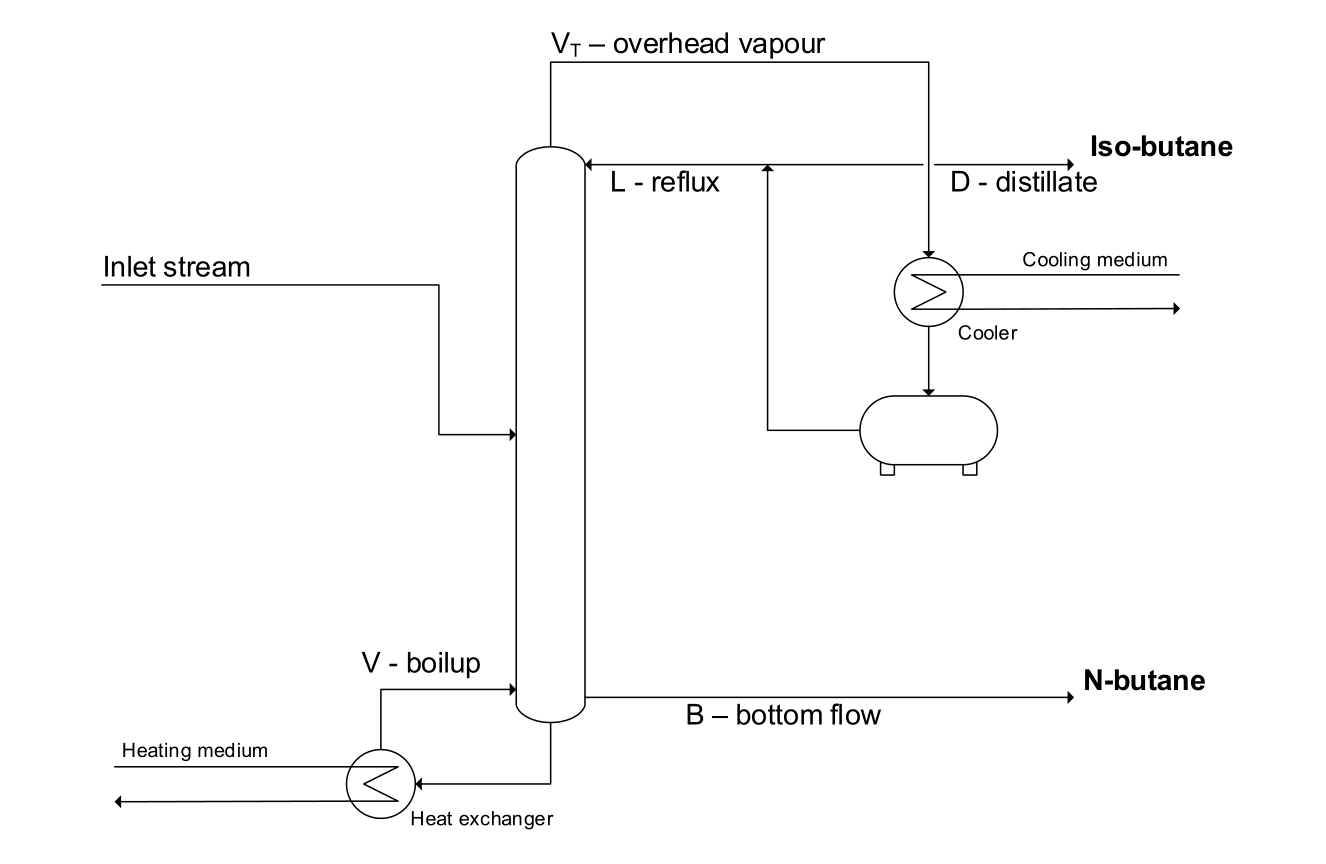
\includegraphics[width=0.95\textwidth]{fig/simplified.png}
	\caption{Simplified model of the plant shown in \autoref{fig:system_full}}
	\label{fig:simplified}
\end{figure}

\begin{figure}[ht!]
	\centering
	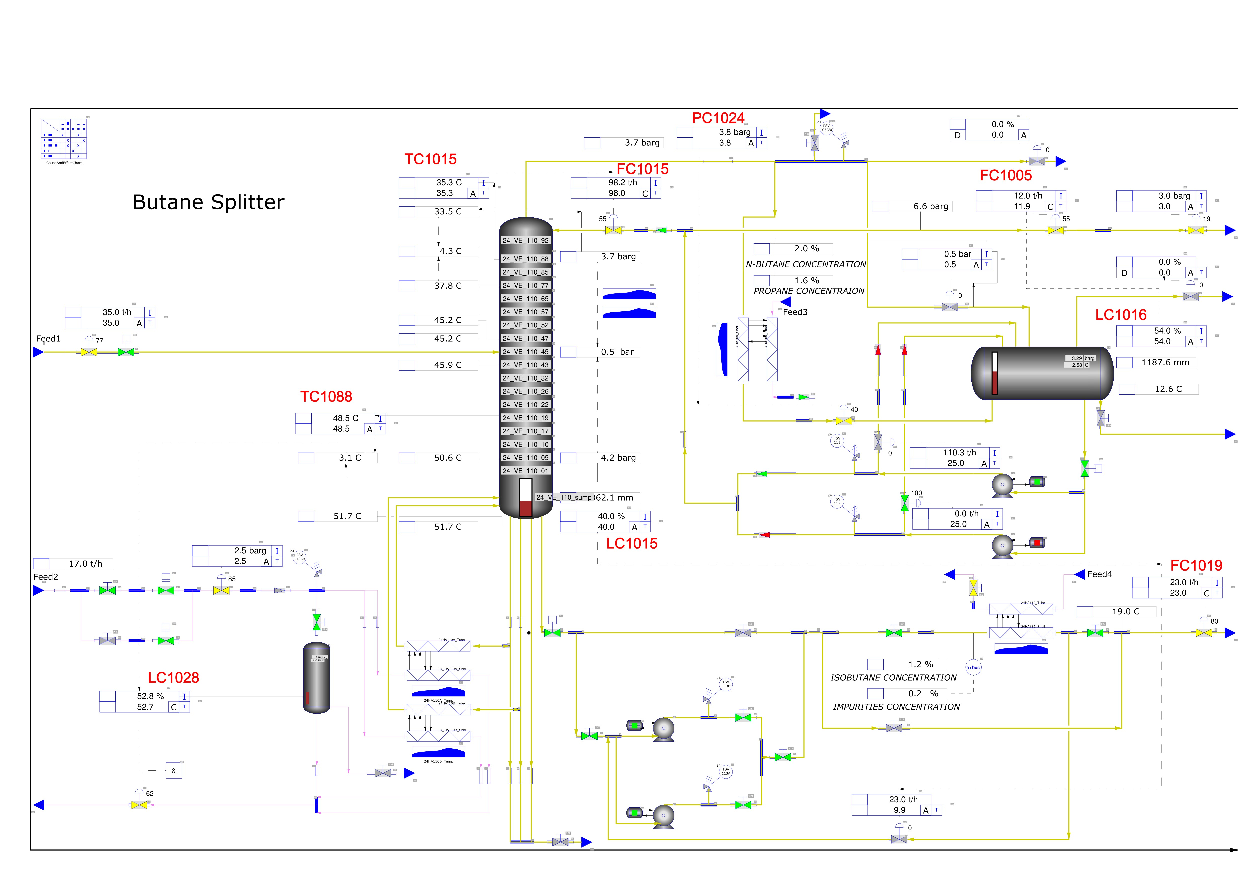
\includegraphics[width=0.95\textwidth]{fig/ButaneSplitter-model-detailed_marked_2.pdf}
	\caption{Full system with controllers numbered with red text}
	\label{fig:system_full}
\end{figure}